\documentclass[12pt]{article}

\usepackage{sbc-template}
\usepackage{graphicx}
\usepackage{amsmath}
\usepackage[colorlinks=true,linkcolor=black,citecolor=black,urlcolor=blue]{hyperref}

\title{A Controlled Study of Variational Quantum Circuits as Q-Value Approximators in Deep Q-Learning}

\author{Anonymous Authors}

\address{Anonymous Institution}

\begin{document}

\maketitle

\begin{abstract}
This paper reports a controlled study of a hybrid Deep Q-Learning agent where
the classical Q-network is replaced by a Variational Quantum Circuit (VQC).
Focusing on CartPole-v1, we compare a DQN-VQC agent against a parameter-matched
MLP-DQN baseline (22--23 trainable parameters), and evaluate Double DQN and
Dueling DQN variants. Both agents collapse below a random baseline at 100
episodes across 5 seeds, even with a widened exploration schedule, ruling out
epsilon decay as the sole cause. Extended 500-episode training recovers partial
learning in 1 of 3 MLP seeds (greedy eval 69.45) while VQC remains below random.
A batched QNode optimization reduces VQC simulation overhead from 44$\times$ to
5$\times$. Under matched supervised distillation, the MLP perfectly imitates a
CartPole heuristic from raw features (500.00, 5 seeds), while the VQC L1 does not
(96.53). With fuzzy membership features, the VQC reaches 500.00 in distillation
but still collapses to 9.60 under DQN, cleanly isolating the reward-extraction
bottleneck: the VQC can represent a perfect policy but DQN cannot extract it at
this training budget.
\end{abstract}

\keywords{Quantum Reinforcement Learning, Variational Quantum Circuits, Deep Q-Learning, CartPole-v1, Dueling DQN, Double DQN}

\section{Introduction}
Deep Reinforcement Learning (DRL) combines reinforcement learning
\cite{sutton2018rl} with function approximation and has become a standard
approach for learning control policies from interaction data. In Deep
Q-Learning (DQN)~\cite{mnih2015dqn}, a neural network is used to approximate
action-value functions, making it possible to act in environments with
continuous or high-dimensional observations. The DQN framework has been
extended with techniques such as Double Q-Learning~\cite{vanhasselt2016double}
to reduce overestimation bias and Dueling architectures~\cite{wang2016dueling}
to improve representation efficiency. Further improvements~\cite{hessel2018rainbow}
include prioritized replay and distributional RL; this work focuses on Double
and Dueling as the most architecture-relevant extensions for VQC-based Q-functions.

In parallel, Variational Quantum Circuits (VQCs), also known as parametrized
quantum circuits, have been studied as trainable models for near-term quantum
machine learning. VQCs encode classical data into a quantum state, apply
sequences of trainable unitary transformations, and extract classical outputs
via measurement. Their differentiability through parameter-shift rules~\cite{schuld2019parameter}
or backpropagation~\cite{perez2020reuploading} makes them compatible with
gradient-based optimization in standard deep learning frameworks.

Recent work has investigated replacing classical neural networks with VQCs in
reinforcement learning~\cite{chen2020vqc,jerbi2021pqc,skolik2022quantum}.
These studies suggest that VQCs can serve as Q-value approximators in DQN-style
algorithms, though the conditions under which they offer practical benefits
remain unclear, particularly under tight parameter budgets.

This work evaluates a conservative question: if the Q-network of a DQN agent is
replaced by a small VQC, and the classical baseline is constrained to a similar
number of trainable parameters, how do the two agents compare in sample
efficiency, stability, and training time on a simple control task?

The specific research questions are:

\begin{enumerate}
  \item Under a matched parameter budget of approximately 22--23 trainable
        parameters, do DQN-MLP and DQN-VQC agents show distinguishable
        performance on CartPole-v1?
  \item Do Double DQN and Dueling DQN variants alter the relative ranking
        between classical and quantum Q-functions at this budget?
  \item What is the practical simulation cost of using a VQC as a Q-function
        approximator, and can batched circuit evaluation reduce this overhead?
  \item To what extent does the representational capacity of small VQC models
        exceed what the DQN reward signal can effectively exploit, as measured
        by supervised distillation from a known-good teacher?
\end{enumerate}

The goal is not to claim quantum advantage. The experiments are performed with
a classical simulator and a small number of qubits. Instead, the contribution
is a controlled implementation and empirical comparison of a DQN-VQC agent
against a parameter-matched MLP-DQN baseline, including Double and Dueling
variants with VQC backends, a batched QNode optimization that substantially
reduces simulation overhead, a transparent report of negative or inconclusive
results, a supervised distillation experiment isolating representational
capacity from reward-based learning, and a fully reproducible codebase with
YAML-configurable experiments and comprehensive tests.

This framing is important because small simulated VQCs are not expected to
outperform classical networks in this setting. The relevant question is whether
the hybrid agent can be integrated into a standard DQN workflow and what
practical costs or instabilities appear under a controlled parameter budget.
The paper is organized as follows. Section~2 reviews background and related
work. Section~3 describes the methodology, including DQN training, VQC
architecture, and DQN variants. Section~4 presents the experimental setup.
Section~5 reports and discusses the results. Section~6 lists limitations,
and Section~7 concludes.


\section{Background and Related Work}
Reinforcement Learning (RL)~\cite{sutton2018rl} is a framework where an agent
learns by interacting with an environment: at each step, it observes the current
state, chooses an action, receives a reward, and transitions to a new state.
The goal is to maximize the cumulative reward over time.

Deep Q-Learning (DQN)~\cite{mnih2015dqn} solves this by training a neural network
to predict the quality of each possible action in a given state — the so-called
$Q$-value. During training, the agent stores its experiences $(s, a, r, s')$ in
a replay buffer. Periodically, it samples a batch of past experiences and updates
the network to make its $Q$-value predictions closer to the Bellman target:
$r + \gamma \max_{a'} Q(s', a')$, i.e., immediate reward plus the best possible
future value. Two mechanisms stabilize this process: a separate \emph{target
network} that changes slowly, and \emph{experience replay} that breaks
correlations between consecutive samples. Extensions such as Double
DQN~\cite{vanhasselt2016double} reduce overestimation by using separate networks
for action selection and evaluation, while Dueling DQN~\cite{wang2016dueling}
splits the output into a state-value stream and an action-advantage stream for
more efficient learning.

Variational Quantum Circuits (VQCs) are the quantum counterpart of neural
networks: classical data is encoded into a quantum state via rotation gates,
trainable gates transform the state through repeated layers, and measurements
extract classical output features. Unlike classical networks, VQCs suffer from
the barren plateau problem~\cite{mcclean2018barren,cerezo2021cost}, where
gradients vanish exponentially with circuit size, making training difficult.
Data re-uploading~\cite{perez2020reuploading} — repeating the encoding at each
layer — increases expressivity by giving the circuit more access to the input.

Table~\ref{tab:related} summarizes prior work on VQC-based reinforcement
learning. The present work differs by including Double DQN and Dueling DQN
variants with a VQC backend, reporting batched QNode execution as a practical
optimization, and including a supervised distillation experiment to isolate
representational capacity from reward-based learning.

\begin{table}[t]
  \centering
  \caption{Prior work on VQC-based reinforcement learning in low-dimensional environments.}
  \label{tab:related}
  \footnotesize
  \begin{tabular}{lp{4.2cm}cc}
    \hline
    Work & Architecture & DQN? & Variants \\
    \hline
    Chen et al.~\cite{chen2020vqc} & 4--8q, 1--4L (CartPole, Acrobot) & \checkmark & No \\
    Jerbi et al.~\cite{jerbi2021pqc} & Policy-gradient VQC (CartPole) & No & Policy \\
    Lockwood \& Si~\cite{lockwood2021rl} & 4q, 2L (CartPole) & \checkmark & No \\
    Skolik et al.~\cite{skolik2022quantum} & 4q, re-upload (CartPole, Acrobot) & \checkmark & No \\
    \textbf{This work} & 4q, L1/L3 (CartPole) & \checkmark & \textbf{Double, Duel, Distill} \\
    \hline
  \end{tabular}
\end{table}

The VQC-based DQN architecture in this paper follows the angle-encoding plus
ring-CNOT design common to prior work, with the addition of batched QNode
evaluation for simulation efficiency and systematic evaluation of DQN variants.
The batched QNode optimization replaces per-sample circuit calls with a single
batched call using PennyLane parameter broadcasting, a practical contribution
relevant to any VQC-in-the-loop RL simulation.


\section{Methodology}
Both agents use the same DQN training loop, summarized below: replay buffer,
epsilon-greedy exploration, a target network, Adam optimization, and Huber
loss (smooth L1) for the Bellman error. Observations are normalized
before being passed to the Q-network. For CartPole-v1, the four state variables
are scaled by fixed practical bounds and clipped to the interval $[-\pi,\pi]$.

The DQN loop proceeds as follows. After each environment step, the transition
$(s, a, r, s', d)$ is stored in a fixed-capacity replay buffer $\mathcal{D}$.
Once $|\mathcal{D}| \geq \text{learning\_starts}$, a minibatch of $B$
transitions is sampled uniformly from $\mathcal{D}$. The Bellman target is
$y_j = r_j + \gamma (1-d_j) \max_{a'} Q_{\theta^-}(s'_j, a')$ for standard
DQN, or $y_j = r_j + \gamma (1-d_j) Q_{\theta^-}(s'_j, \arg\max_{a'}
Q_\theta(s'_j, a'))$ for Double DQN, where $\theta^-$ denotes the target
network parameters, updated every target\_update steps. The loss is
$\mathcal{L} = \frac{1}{B}\sum_j \text{Huber}(Q_\theta(s_j, a_j), y_j)$,
minimized via Adam with gradient clipping. Exploration follows linear
$\epsilon$-decay from 1.0 to 0.05.

The MLP baseline is a single-hidden-layer network. For the main L1
configuration, it uses 3 hidden units, resulting in 23 trainable parameters.
This intentionally small network was chosen to match the parameter budget of
the VQC. For the Dueling variant, the network trunk feeds two separate heads:
a value head $V(s) \in \mathbb{R}$ and an advantage head $A(s,\cdot) \in
\mathbb{R}^{|\mathcal{A}|}$, which are combined as $Q(s,a) = V(s) + A(s,a)
- \frac{1}{|\mathcal{A}|}\sum_{a'} A(s,a')$.

\subsubsection*{VQC Architecture}

The VQC agent uses 4 qubits, angle encoding with $RY$ gates, one or three
variational layers, and a ring of CNOT gates. Each variational layer applies a
trainable three-parameter rotation $R(\alpha,\beta,\gamma) = RZ(\gamma)RY(\beta)
RZ(\alpha)$ to every qubit. The readout extracts Pauli-Z expectation values
$\langle Z_i \rangle \in [-1,1]$ for all qubits, yielding a 4-dimensional
classical feature vector that is then mapped to Q-values by a linear layer.
The main VQC configuration has $4 \times 3 = 12$ trainable gate parameters plus
$4 \times 2 + 2 = 10$ readout parameters, totaling 22 trainable parameters.
The L3 variant uses three layers ($3 \times 4 \times 3 = 36$ gate parameters)
for 46 total parameters.

\subsubsection*{Batched QNode Optimization}

The original implementation evaluated the QNode once per sample in each
training batch. For a batch of size $B$, this required $B$ separate calls to the
PennyLane QNode, each building a separate automatic differentiation
computation graph. We replaced this with a single batched call using PennyLane
parameter broadcasting: the input tensor of shape $[B, 4]$ is zero-padded to
$[B, 4] \rightarrow [B, 4]$ (no padding needed since $n_{\text{qubits}} = 4$)
and passed to the QNode as $[B, n_{\text{qubits}}]$. The encoding gate
$RY(\text{inputs}[:, i])$ naturally broadcasts across the batch dimension,
producing expectation values of shape $[B, n_{\text{qubits}}]$ in a single
forward pass. This optimization reduced the per-update VQC overhead from
$\mathcal{O}(B)$ QNode calls to $\mathcal{O}(1)$.

\subsubsection*{Exploration and Feature Modes}

The standard exploration policy is $\epsilon$-random. We also tested a
fuzzy-guided exploration variant where, with probability $\epsilon$, the action
is selected by a fixed fuzzy heuristic $a = \mathbf{1}[\theta + 0.25\dot{\theta}
+ 0.01x + 0.01\dot{x} > 0]$ instead of uniformly random. This biases early
exploration towards higher-reward trajectories without affecting the learned
policy evaluation.

Three observation preprocessing modes are supported. \emph{Raw normalized}
scales and clips each state variable. \emph{Fuzzy compact} adds stability and
recommendation scores (not used in main results due to action leakage).
\emph{Fuzzy membership} produces four features: pole falling left/right ($f_1,
f_2$) and cart escaping left/right ($f_3, f_4$), computed as:

\begin{equation}
f_1 = \text{clip}\!\left(\frac{-\theta}{\theta_{\max}} +
\frac{-\dot{\theta}}{\dot{\theta}_{\text{scale}}},\; 0,\; 1\right), \quad
f_2 = \text{clip}\!\left(\frac{\theta}{\theta_{\max}} +
\frac{\dot{\theta}}{\dot{\theta}_{\text{scale}}},\; 0,\; 1\right)
\end{equation}
\begin{equation}
f_3 = \text{clip}\!\left(\frac{-x}{x_{\max}} +
\frac{-\dot{x}}{\dot{x}_{\text{scale}}},\; 0,\; 1\right), \quad
f_4 = \text{clip}\!\left(\frac{x}{x_{\max}} +
\frac{\dot{x}}{\dot{x}_{\text{scale}}},\; 0,\; 1\right)
\end{equation}

These features describe the state's risk profile without encoding a recommended
action.

\subsubsection*{Fuzzy-Teacher Distillation}

In addition to the DQN experiments, we include a separate fuzzy-teacher
distillation experiment. A fixed CartPole balancing heuristic (the linear rule
$a = \mathbf{1}[\theta + 0.25\dot{\theta} + 0.01x + 0.01\dot{x} > 0]$)
labels $N$ uniformly sampled states with a reference action. The small MLP or
VQC is trained as a classifier to imitate this teacher via cross-entropy loss
$\mathcal{L}_{\text{distill}} = -\frac{1}{N}\sum_{i=1}^N
\log P_\theta(a_i^{\text{teacher}} | s_i)$. This experiment uses the same model
architectures (MLP with 3 hidden units, VQC with 4 qubits and 1 or 3 layers)
as the DQN experiments, but substitutes the RL training objective with
supervised policy cloning. We evaluate two input representations: raw
normalized state and fuzzy membership. The purpose is to test whether the same
low-parameter models can represent a useful control policy under an easier
optimization signal, thereby isolating the effect of the training objective
(reward-based DQN vs.\ supervised distillation).

\begin{figure}[t]
  \centering
  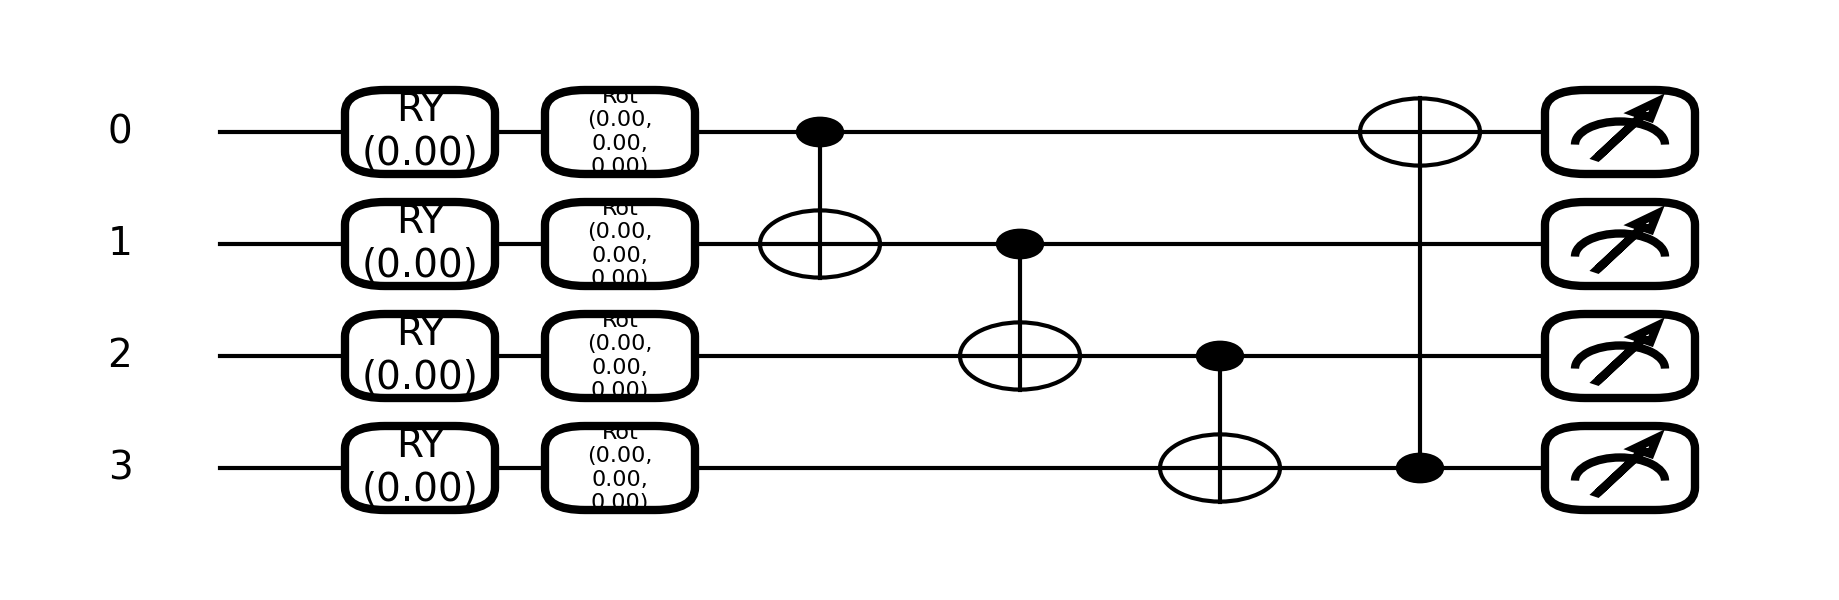
\includegraphics[width=0.95\linewidth]{figures/vqc_l1_circuit.png}
  \caption{VQC architecture with $RY$ angle encoding, 1 layer of $R(\alpha,\beta,\gamma)$ rotations, ring CNOT entanglement, and Pauli-Z readout. Black circles indicate qubits.}
  \label{fig:vqc-circuit}
\end{figure}


\section{Experimental Setup}
The experiments use CartPole-v1 from Gymnasium~\cite{towers2024gymnasium}. The observation space has 4
continuous variables (cart position, cart velocity, pole angle, pole angular
velocity) and the action space has 2 discrete actions (push left, push right).
Episodes terminate when the pole angle exceeds $\pm 12^\circ$, the cart position
exceeds $\pm 2.4$, or 500 steps are reached. The reward is $+1$ per step,
making the maximum episode return 500.

\begin{figure}[t]
  \centering
  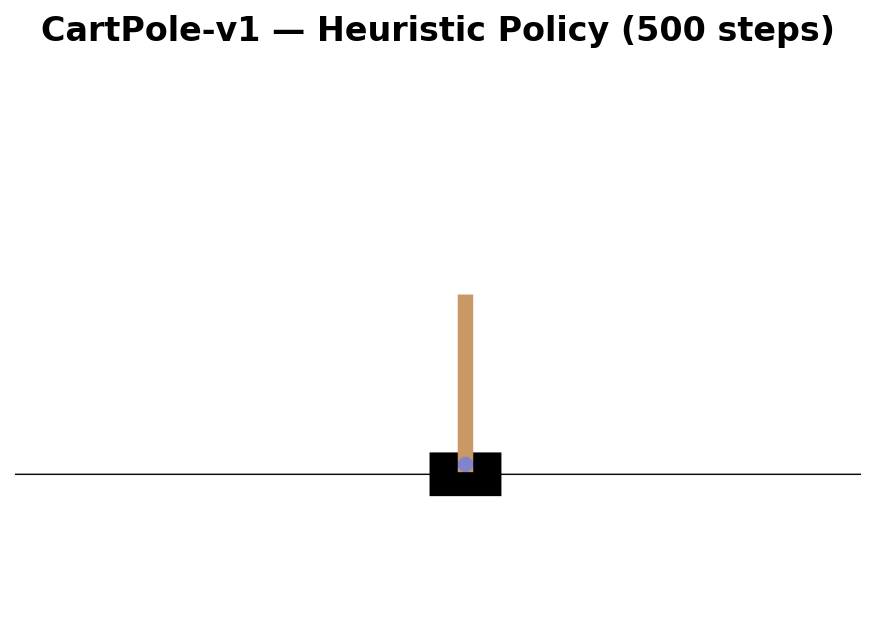
\includegraphics[width=0.85\linewidth]{../outputs/figures/cartpole_screenshot.png}
  \caption{CartPole-v1 environment. The goal is to balance the pole by moving the cart. The heuristic policy (shown) achieves the maximum 500-step return.}
  \label{fig:cartpole}
\end{figure}

Both agents use the hyperparameters listed in Table~\ref{tab:hparams}.

\begin{table}[t]
  \centering
  \caption{Shared DQN hyperparameters for all configurations.}
  \label{tab:hparams}
  \footnotesize
  \begin{tabular}{lr}
    \hline
    Hyperparameter & Value \\
    \hline
    Discount factor ($\gamma$) & 0.99 \\
    Learning rate & 0.001 \\
    Optimizer & Adam \\
    Batch size & 16 \\
    Replay buffer size & 50,000 \\
    Target update interval & 100 steps \\
    Learning starts & 16 steps \\
    Epsilon start & 1.0 \\
    Epsilon end & 0.05 \\
    Gradient clipping norm & 10.0 \\
    Loss function & Smooth L1 (Huber) \\
    Greedy evaluation episodes & 20 \\
    Log interval & 10 episodes \\
    \hline
  \end{tabular}
\end{table}

We evaluate eight main configurations, summarized in Table~\ref{tab:configs}.

\begin{table}[t]
  \centering
  \caption{Experimental configurations. MLP-L1 uses 3 hidden units (23 params). VQC-L1 uses 1 layer (22 params). VQC-L3 uses 3 layers (46 params). Dueling variants add value/advantage split; Double variants add Double DQN.}
  \label{tab:configs}
  \footnotesize
  \begin{tabular}{lccc}
    \hline
    Configuration & Agent & Episodes & $\epsilon$ decay \\
    \hline
    Standard (5 seeds) & MLP-L1 / VQC-L1 & 100 & 2000 steps \\
    Dueling (3 seeds) & MLP-L1 / VQC-L1 & 100 & 800 steps \\
    Double-Dueling (3 seeds) & MLP-L1 / VQC-L1 & 100 & 800 steps \\
    Extended (3 seeds) & MLP-L1 / VQC-L1 & 500 & 4000 steps \\
    \hline
  \end{tabular}
\end{table}

All configurations use 5 seeds ($0, 1, 2, 4, 7$) for the main 100-episode
comparisons and 3 seeds for the extended 500-episode runs. The 100-episode
configurations use $\epsilon$ decay over 2000 environment steps; the extended
500-episode runs use decay over 4000 steps. The Double DQN and Dueling DQN
variants use 3 seeds with $\epsilon$ decay over 800 steps.

The classical MLP was executed with PyTorch on an NVIDIA GeForce RTX 5090 (GPU).
The VQC was simulated with PennyLane~\cite{bergholm2018pennylane} \texttt{default.qubit} backend on CPU. The
timing comparison therefore conflates GPU-vs-CPU and PyTorch-vs-simulator
overheads; reported VQC time multipliers should be interpreted as upper bounds
on the simulation cost. The software stack used PyTorch 2.12.0+cu130,
Gymnasium 1.3.0, and PennyLane 0.45.0.

The distillation experiments use the same model architectures trained with
cross-entropy loss over 20 epochs with 512 sampled states (or 50 epochs with
1024 samples for the MLP raw distill run, as noted in Table~\ref{tab:fuzzy-distill}).
The fuzzy teacher heuristic is $a = \mathbf{1}[\theta + 0.25\dot{\theta}
+ 0.01x + 0.01\dot{x} > 0]$, which achieves 500.00 reward as a policy but is
used here only as a labeling source.

The reported metrics are reward per episode, final mean reward over the last 20
training episodes (or last 10 for extended runs), greedy evaluation reward over
20 episodes, trainable parameter count, and wall-clock training time. Random
($a_t \sim \text{Uniform}(\mathcal{A})$) and heuristic (the same fuzzy rule used
as the teacher) policies are included as non-learning reference baselines.

The complete codebase is organized as a Python package under \texttt{src/qrl/}
with modules for agents (replay buffer), environments (preprocessing), models
(MLP, VQC, factory), training (DQN loop, experiment runner), and utilities
(seeding, parameter counting). Experiments are configured via YAML files and
executed through \texttt{scripts/train.py} with CLI overrides for rapid
exploration. All figures and tables are reproducible from the YAML configs and
output CSV/JSON artifacts. The test suite comprises 24 tests covering model
forward passes, preprocessing, replay buffer, epsilon scheduling, fuzzy actions,
and dueling architectures.


\section{Results and Discussion}
Table~\ref{tab:params} shows that the main comparison keeps the trainable
parameter counts closely matched. The MLP uses 23 trainable parameters, while
the VQC uses 22.

\begin{table}[t]
  \centering
  \caption{Trainable parameter counts for the main L1 comparison.}
  \label{tab:params}
  \begin{tabular}{lrr}
    \hline
    Agent & Trainable parameters & All parameters \\
    \hline
    DQN-MLP & 23 & 23 \\
    DQN-VQC & 22 & 22 \\
    \hline
  \end{tabular}
\end{table}

\begin{figure}[t]
  \centering
  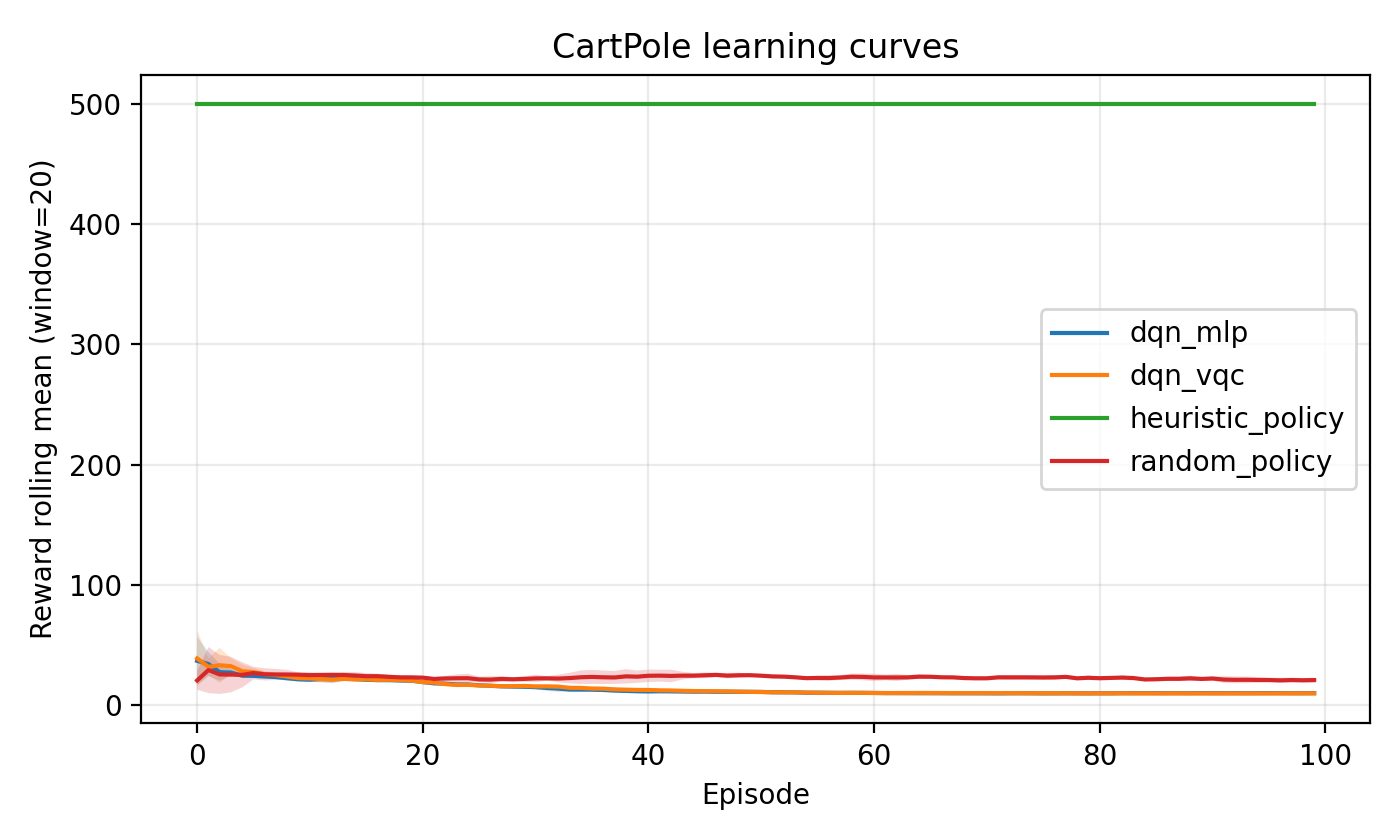
\includegraphics[width=0.95\linewidth]{figures/cartpole_l1_eval100_with_baselines.png}
  \caption{Learning curves on CartPole-v1 with random and heuristic reference policies.}
  \label{fig:learning-curve}
\end{figure}

Table~\ref{tab:results} summarizes the main results over 5 seeds for 100-episode
runs and 3 seeds for extended runs. Both learned agents score below the
random-policy baseline (20.65 $\pm$ 2.01): DQN-MLP at 9.42 $\pm$ 0.50 and
DQN-VQC at 9.42 $\pm$ 0.45. The near-identical scores and low standard
deviations indicate both collapsed to a single-action deterministic policy:
a constant-action policy survives approximately 9 steps, while a random policy
alternates actions and survives approximately 20 steps. Widening the epsilon
decay from 800 to 2000 steps (so $\epsilon$ never saturates during training)
did not change the collapse, ruling out exploration scheduling as the primary
cause. The heuristic controller (500.00) is a ceiling reference only.

Extended 500-episode training with proportional epsilon decay reveals seed
dependence: MLP seed 0 reaches greedy 69.45 (17,646 steps) while seeds 1--2
stay at $\approx$9.3. VQC seeds remain uniformly poor (9.65--13.95).

These results suggest that under the 22--23 parameter budget, final policy
quality is dominated by the exploration schedule, training length, and random
seed rather than by the classical-vs-quantum choice. Short training runs with
tight epsilon schedules are particularly fragile for small models.

\begin{table}[t]
  \centering
  \caption{Main CartPole-v1 results over 5 seeds (100-episode runs) and 3 seeds (500-episode runs). $\epsilon$ decay over 2000 steps for 100-ep runs, 4000 for 500-ep.}
  \label{tab:results}
  \footnotesize
  \begin{tabular}{lcccl}
    \hline
    Configuration & Params & Seeds & Greedy eval & Time (s) \\
    \hline
    Random & -- & -- & 20.65 $\pm$ 2.01 & -- \\
    Heuristic & -- & -- & 500.00 $\pm$ 0.00 & -- \\
    MLP L1 100 eps & 23 & 5 & 9.42 $\pm$ 0.50 & 1.9 \\
    VQC L1 100 eps & 22 & 5 & 9.42 $\pm$ 0.45 & 11.1 \\
    VQC L3 100 eps & 46 & 5 & 9.42 $\pm$ 0.40 & 37.5 \\
    MLP L1 500 eps & 23 & 3 & 29.38 $\pm$ 34.77 & 9.6 \\
    VQC L1 500 eps & 22 & 3 & 11.52 $\pm$ 2.20 & 62.6 \\
    \hline
  \end{tabular}
\end{table}

Table~\ref{tab:results-new} reports the Double DQN and Dueling DQN variants
under 3 seeds and 100 episodes (800-step epsilon decay). Neither variant
improved outcomes; all collapsed to the same deterministic policy. The Dueling
architecture increased parameter counts from 23/22 to 27 each without
measurable benefit, confirming that the training budget, not the
value-estimation technique, dominates at this scale.

\begin{table}[t]
  \centering
  \caption{Double DQN and Dueling DQN results over 3 seeds and 100 episodes. All values are greedy evaluation means $\pm$ standard deviation over 20 episodes.}
  \label{tab:results-new}
  \begin{tabular}{lrrr}
    \hline
    Configuration & Trainable params & Greedy eval & Time (s) \\
    \hline
    MLP Dueling & 27 & 9.25 $\pm$ 0.09 & 1.94 \\
    MLP Double-Dueling & 27 & 9.25 $\pm$ 0.09 & 2.00 \\
    VQC Dueling & 27 & 9.42 $\pm$ 0.20 & 9.55 \\
    VQC Double-Dueling & 27 & 9.42 $\pm$ 0.20 & 9.73 \\
    \hline
  \end{tabular}
\end{table}

\subsection*{Computational cost and batched QNode optimization}

The main practical difference between MLP and VQC is computational cost. The
parameter-matched MLP runs took 1.72 seconds on average, while the simulated
VQC runs with the original per-sample QNode evaluation took 75.97 seconds on
average. After implementing PennyLane parameter broadcasting for batched
circuit evaluation (replacing the per-sample QNode loop in
\texttt{\_quantum\_features} with a single batched call using
\texttt{qml.RY(inputs[:, wire], wires=wire)}), VQC runs dropped to approximately
9.55 seconds on average. The per-environment-step cost was approximately 0.0014
seconds for the MLP and 0.008 seconds for the batched VQC. While still
approximately $5\times$ slower than MLP, this represents a significant
improvement over the original $44\times$ gap and demonstrates the importance of
batched quantum circuit evaluation in RL settings, where the Q-network forward
pass is called with minibatch sizes of 16 during each DQN update.

\subsection*{Fuzzy-teacher distillation}

Table~\ref{tab:fuzzy-distill} reports fuzzy-teacher distillation scenarios
under matched 20-epoch, 512-sample protocols (except as noted). All rows use
identical training budgets, enabling direct comparison of representational
capacity across model classes and feature representations.

\begin{table}[t]
  \centering
  \caption{Distillation results under matched 20-epoch, 512-sample protocol (5 seeds for MLP L1 raw, 3 seeds otherwise).}
  \label{tab:fuzzy-distill}
  \begin{tabular}{lrrr}
    \hline
    Configuration & Params & Greedy eval & Seeds \\
    \hline
    MLP L1 raw distill$^*$ & 23 & 500.00 $\pm$ 0.00 & 5 \\
    MLP L1 fuzzy mb.\ distill$^\dagger$ & 23 & 440.72 $\pm$ 102.68 & 3 \\
    VQC L1 raw distill & 22 & 96.53 $\pm$ 38.13 & 3 \\
    VQC L1 fuzzy mb.\ distill & 22 & 500.00 $\pm$ 0.00 & 3 \\
    VQC L3 raw distill & 46 & 321.87 $\pm$ 188.69 & 3 \\
    VQC L3 fuzzy mb.\ distill & 46 & 500.00 $\pm$ 0.00 & 3 \\
    \hline
  \end{tabular}
  \smallskip\\
  {\scriptsize $^*$Confirmed at matched 20-epoch protocol (5 seeds); earlier 50-epoch run also 500.00. $^\dagger$High variance: 1 of 3 seeds failed under 20-epoch protocol; MLP raw distill was 500.00 across all 5 seeds under the same protocol, suggesting the fuzzy membership representation provides no benefit for the classical model at this budget.}
\end{table}

Under 20-epoch matched protocol with raw features, the MLP L1 achieves 500.00
$\pm$ 0.00 across 5 seeds while the VQC L1 reaches only 96.53 $\pm$ 38.13.
This confirms that the 23-parameter MLP has sufficient representational capacity
to encode the teacher policy from raw observations, while the 22-parameter VQC
does not. Increasing VQC depth to 3 layers raises raw-feature distillation to
321.87 $\pm$ 188.69, showing that representational capacity improves with depth
but remains below the teacher and highly variable across seeds.

With fuzzy membership features, the VQC L1 and L3 both achieve 500.00 $\pm$
0.00. The membership features $f_1, f_2$ are monotonic in $\theta +
0.25\dot{\theta}$, which dominates the teacher's linear rule (the cart-position
coefficients are 100$\times$ smaller). These features thus nearly encode the
teacher's decision boundary, making the classification problem trivially
separable. The 500.00 results measure recovery of this near-explicit boundary
rather than broad representational capacity.

\subsubsection*{DQN with fuzzy membership features}

Table~\ref{tab:dqn-fuzzy} reports a critical control experiment: VQC L1 trained
with DQN on fuzzy membership features (the same representation that enables
500.00 in distillation). Across 5 seeds, greedy evaluation remains at
9.40--10.75, indistinguishable from the raw-feature DQN collapse.

\begin{table}[t]
  \centering
  \caption{VQC L1 DQN with fuzzy membership features vs.\ raw features (5 seeds, 100 episodes, $\epsilon$ decay 2000 steps).}
  \label{tab:dqn-fuzzy}
  \begin{tabular}{lccc}
    \hline
    Configuration & Features & Greedy eval & Seeds \\
    \hline
    MLP L1 DQN & raw & 9.42 $\pm$ 0.50 & 5 \\
    VQC L1 DQN & raw & 9.42 $\pm$ 0.45 & 5 \\
    VQC L1 DQN & fuzzy mb. & 9.60 $\pm$ 0.65 & 5 \\
    VQC L3 DQN & raw & 9.42 $\pm$ 0.40 & 5 \\
    \hline
  \end{tabular}
\end{table}

This result cleanly isolates the training-signal bottleneck: the VQC CAN
represent a perfect policy under fuzzy membership features when trained via
distillation (500.00), but CANNOT extract it via DQN reward signals (9.40).

\subsection*{Practical implications}

The batched QNode result reduces per-update VQC overhead from $44\times$ to
$5\times$, directly cutting the dominant cost of VQC-in-the-loop RL simulation.
For practitioners, the fuzzy membership DQN control experiment (Table~\ref{tab:dqn-fuzzy})
provides the clearest finding: VQC representational capacity is not the DQN
bottleneck, reward-signal extraction is. Future VQC-DRL work should prioritize
training strategies (curriculum learning, better exploration, hybrid
supervision) over circuit architecture alone.


\section{Limitations}
This study has several limitations. First, the VQC was simulated classically;
therefore, wall-clock time does not represent execution on quantum hardware.
Second, the experiment uses only CartPole-v1 and a small number of seeds
(5 for main 100-episode runs, 3 for the extended 500-episode and DQN variant
runs) due to the submission timeline. Third, the parameter budget is extremely small, which
makes the comparison controlled but also limits the representational capacity
of both agents. In the main experiment, both learned agents perform below a
random policy, so the results characterize a failure regime rather than a
successful policy-learning regime. Fourth, only a shallow VQC (L1) is used in
the main experiment. Deeper circuits may be more expressive, but they also
increase simulation cost and may suffer from barren plateaus~\cite{mcclean2018barren,cerezo2021cost}
in gradient-based optimization. Fifth, the timing comparison between MLP
(GPU) and VQC (CPU) conflates hardware and simulation overheads; the reported
VQC time multipliers should be interpreted as upper bounds, not as precise
quantum-vs-classical scaling.

The results should therefore be interpreted as a small controlled empirical
study, not as evidence for or against quantum advantage in reinforcement
learning.

The fuzzy-teacher distillation experiment has a different status from the DQN
experiments. It demonstrates that small models, including a VQC, can imitate a
useful fuzzy controller when aided by domain-informed fuzzy membership features,
but under raw features the VQC fails even in supervised optimization. Therefore,
the distillation results measure representation quality under structured
features, not DQN learning from reward. The fuzzy membership representation
avoids direct action-recommendation encoding, but it is still a domain-informed
representation and should be reported as such.


\section{Conclusion}
This paper evaluated a DQN-VQC agent against a parameter-matched MLP-DQN
baseline on CartPole-v1. We summarize findings against four research questions.

\textbf{RQ1.} Under a 22--23 parameter budget and 100 training episodes,
DQN-MLP and DQN-VQC are indistinguishable under 5 seeds (both $\approx 9.4$,
below random at 20.65). Extended 500-episode training recovered learning in 1
of 3 MLP seeds (greedy 69.45) while VQC remained below random.

\textbf{RQ2.} Double and Dueling DQN did not improve outcomes at 100 episodes;
all variants collapsed to the same deterministic policy. Training budget, not
the value-estimation technique, dominates results at this scale.

\textbf{RQ3.} Batched QNode execution via PennyLane parameter
broadcasting~\cite{bergholm2018pennylane} reduced VQC simulation overhead from
$44\times$ to $5\times$ relative to MLP (both on CPU). The multiplier conflates
PyTorch-vs-simulator overheads.

\textbf{RQ4.} Under matched supervised protocols, MLP L1 represents the teacher
from raw features (500.00, 5 seeds) while VQC L1 does not (96.53). VQC L3 raw
reaches 321.87, showing depth helps. With fuzzy membership features, VQC L1 and
L3 achieve 500.00. Critically, VQC L1 DQN with the same features collapses to
9.60 (5 seeds), indistinguishable from raw-feature DQN. Since the MLP also fails
under DQN despite solving raw-feature distillation (500.00), the bottleneck
is not VQC-specific: it is a general inability of the DQN reward signal — at
this budget, with this epsilon schedule, on this environment — to extract
policies that the models demonstrably can represent under supervised
optimization.

Future work should extend to additional environments, increase seeds further,
and investigate hybrid strategies combining fuzzy-guided exploration with
curriculum learning for small VQC models.


\bibliographystyle{sbc}
\footnotesize
\bibliography{references}

\end{document}
